\documentclass{tufte-handout}

%\usepackage{scrextend} 
%\changefontsizes[20pt]{12pt}

\geometry{a4paper,landscape,left=24.8mm,top=27.4mm,headsep=2\baselineskip,textwidth=164mm,marginparsep=8.2mm,marginparwidth=82mm,textheight=34\baselineskip,headheight=\baselineskip}

%\geometry{showframe}% for debugging purposes -- displays the margins

\usepackage{amsmath,amsthm,amssymb}
\theoremstyle{definition}
\newtheorem{theorem}{Theorem}[section]
\newtheorem*{theorem*}{Theorem}
\newtheorem{corollary}[theorem]{Corollary}
\newtheorem{lemma}[theorem]{Lemma} 
\newtheorem{proposition}[theorem]{Proposition}
\newtheorem{conj}[theorem]{Conjecture}
\newtheorem{defn}[theorem]{Definition}
\newtheorem{fact}[theorem]{Fact} 
\newtheorem{example}[theorem]{Example} 
\newtheorem{examples}[theorem]{Examples}
\newtheorem{example*}[theorem]{Example*}
\newtheorem{examples*}[theorem]{Examples*}
\newtheorem{remark}[theorem]{Remark}
\newtheorem{remark*}[theorem]{Remark*}
\newtheorem{question}[theorem]{Question}
\newtheorem{assumption}[theorem]{Assumption}
\newtheorem{conjecture}[theorem]{Conjecture}
\newtheorem{convention}[theorem]{Convention}
\newtheorem{justification}[theorem]{Justification} 
\newtheorem{construction}[theorem]{Construction}
\newtheorem{rem}[theorem]{Reminder}
\newtheorem{intuition}[theorem]{Intuition}
\newtheorem{term}[theorem]{Terminology}

\usepackage{tikz-cd}
\usepackage{macros/tikzfig}
\usepackage{macros/quiver}
\input{macros/toprel.tikzstyles}

% Set up the images/graphics package
\usepackage{graphicx}
\setkeys{Gin}{width=\linewidth,totalheight=\textheight,keepaspectratio}
\graphicspath{{graphics/}}

\title{The Category of Topological Relations}
\author[V.W.]{Vincent Wang-Ma\'{s}cianica}
\date{\today}

% The following package makes prettier tables.  We're all about the bling!
\usepackage{booktabs}

% The units package provides nice, non-stacked fractions and better spacing
% for units.
\usepackage{units}

% The fancyvrb package lets us customize the formatting of verbatim
% environments.  We use a slightly smaller font.
\usepackage{fancyvrb}
\fvset{fontsize=\normalsize}

% Small sections of multiple columns
\usepackage{multicol}

% Squares
\usepackage{stix}

% Provides paragraphs of dummy text
\usepackage{lipsum}

% These commands are used to pretty-print LaTeX commands
\newcommand{\doccmd}[1]{\texttt{\textbackslash#1}}% command name -- adds backslash automatically
\newcommand{\docopt}[1]{\ensuremath{\langle}\textrm{\textit{#1}}\ensuremath{\rangle}}% optional command argument
\newcommand{\docarg}[1]{\textrm{\textit{#1}}}% (required) command argument
\newenvironment{docspec}{\begin{quote}\noindent}{\end{quote}}% command specification environment
\newcommand{\docenv}[1]{\textsf{#1}}% environment name
\newcommand{\docpkg}[1]{\texttt{#1}}% package name
\newcommand{\doccls}[1]{\texttt{#1}}% document class name
\newcommand{\docclsopt}[1]{\texttt{#1}}% document class option name

\begin{document}

\maketitle% this prints the handout title, author, and date

\begin{fullwidth}
\section{Introduction}
\end{fullwidth}

\chapter{Topological Relations}

\marginnote{
\begin{rem}[Topological Space]
A \emph{topological space} is a pair $(X,\tau)$, where $X$ is a set, and $\tau \subset \mathcal{P}(X)$ are the \emph{open sets} of $X$, such that:
\begin{description}
    \item["nothing" and "everything" are open]  \[\varnothing,X \in \tau\]
    \item[Arbitrary unions of opens are open] \[\{ U_i : i \in I \} \subseteq \tau \Rightarrow \bigcup\limits_{i \in I} U_i \in \tau \]
    \item[Finite intersections of opens are open] $n \in \mathbb{N}$: \[U_1,\cdots, U_n \in \tau \Rightarrow \bigcap\limits_{1\cdots, i , \cdots n} U_i \in \tau\]
\end{description}
\end{rem}
}

\marginnote{
\begin{rem}[Relational Converse]
Recall that a relation $R: S \rightarrow T$ is a subset $R \subseteq S \times T$. \[R^\dag : T \rightarrow S := \{ (t,s) : (s,t) \in R \}\]
\end{rem}
}
\begin{defn}[Topological Relation]\label{defn:toprelation}
A topological relation $R: (X,\tau) \rightarrow (Y,\sigma)$ is a relation $R: X \rightarrow Y$ such that \[U \in \sigma \Rightarrow R^{\dag}(U) \in \tau\] where $\dag$ denotes the relational converse.
\end{defn}

For shorthand, we denote the topology $(X,\tau)$ as $X^{\tau}$. As special cases, we denote the discrete topology on $X$ as $X^{\bullet}$, and the indiscrete topology $X^{\circ}$.

\newpage

\begin{fullwidth}

\section{Topological Relations by examples}

Let's consider three topological spaces and examine the topological relations between them. This way we can build up intuitions, and prove some tool results in the process.

The \textbf{singleton space} consists of a single point which is both open and closed. We denote this space $\bullet$. Concretely, the underlying set and topology is
\[(\{\star\} \ , \ \{\{\star\},\varnothing\})\] 
\ctikzfig{testspaces/singleton}

The \textbf{Sierpi\'{n}ski space} consists of two points, one of which (in yellow) is open, and the other (in cyan) is closed. We denote this space $\mathcal{S}$. Concretely, the underlying set and topology is:
\[\big( \{0,1\} \ , \ \{ \varnothing, \{ 1 \} , \{ 0,1\} \} \big)\]
\ctikzfig{testspaces/sierpinski}

The \textbf{unit square} has $[0,1] \times [0,1]$ as its underlying set.  Open sets are "blobs" painted with open balls. Points, lines, and bounded shapes are closed. We denote this space $\blacksquare$.
\ctikzfig{testspaces/unitsquare}
\end{fullwidth}

\newthought{$\bullet \rightarrow \bullet$:} There are two relations from the singleton to the singleton; the identity relation $\{ (\bullet,\bullet) \}$, and the empty relation $\varnothing$. Both are topological.

\newthought{$\bullet \rightarrow \mathcal{S}$:} There are four relations from the singleton to the Sierpi\'{n}ski space, corresponding to the subsets of $\mathcal{S}$. All of them are topological.


\newthought{$\mathcal{S} \rightarrow \bullet$:}
\marginnote{
\begin{example}[A nontopological relation]\label{ex:nontop}
The relation $\{(0,\bullet)\} \subset \mathcal{S} \times \bullet$ is not a topological relation: the preimage of the open set $\{\bullet\}$ under this relation is the non-open set $\{0\}$.
\end{example}
}
There four candidate relations from the Sierpi\'{n}ski space to the singleton, but as we see in Example \ref{ex:nontop}, not all of them are topological.

\newthought{Now we need some abstraction.} We cannote study the topological relations between the singleton and the unit square case by case. We discover that topological relations out of the singleton indicate arbitrary subsets, and that topological relations into the singleton indicate arbitrary opens.
\marginnote{
\begin{term}
Call a topological relation $\bullet \rightarrow X^\tau$ a \textbf{state} of $X^\tau$, and a topological relation $X^\tau \rightarrow \bullet$ a \textbf{test} of $X^\tau$.
\end{term}

\begin{proposition}\label{prop:states}
States $R: \bullet \rightarrow X^{\tau}$ correspond with subsets of $X$.
\begin{proof}
The preimage $R^\dag(U)$ of a (non-$\varnothing$) open $U \in \tau$ is $\star$ if $R(\star) \cap U$ is nonempty, and $\varnothing$ otherwise. Both $\star$ and $\varnothing$ are open in $\{\star\}^{\bullet}$. $R(\star)$ is free to specify any non-$\varnothing$ subset of $X$. The empty relation handles $\varnothing$ as an open of $X^{\tau}$.
\end{proof}
\end{proposition}

\begin{proposition}\label{prop:tests}
Tests $R: X^\tau \rightarrow \bullet$ correspond with open sets $U \in \tau$.
\begin{proof}
The preimage $R^\dag(\star)$ of $\star$ must be an open set of $X^\tau$ by definition \ref{defn:toprelation}. $R^\dag(\star)$ is free to specify any open set of $X^{\tau}$.
\end{proof}
\end{proposition}
}

\newthought{$\bullet \rightarrow \blacksquare$:} Proposition \ref{prop:states} tells us that there are as many topological relations from the singleton to the unit square as there are subsets of the unit square.

\newthought{$\blacksquare \rightarrow \bullet$:} Proposition \ref{prop:tests} tells us that there are as many topological relations from the unit square to the singleton as there are open sets of the unit square.

\newthought{There are 16 candidate relations $\mathcal{S} \rightarrow \mathcal{S}$ to check.} A case-by-case approach won't scale, so we could instead identify the building blocks of topological relations with the same source and target space.

\newthought{Which relations $X^\tau \rightarrow Y^\sigma$ are always continuous?}

\newthought{The empty relation is always continuous.}
\marginnote{
    \begin{rem}[Empty relation]
    The \textbf{empty relation} $X \rightarrow Y$ relates nothing. It is defined:
    \[ \varnothing \subset X \times Y\]
    \end{rem}
}
\begin{proposition}
\label{prop:emptyrel}
\begin{proof}
The preimage of the empty relation is always $\varnothing$, which is open by definition.
\end{proof}
\end{proposition}

\newthought{Full relations are always continuous}
\marginnote{
    \begin{rem}[Full relation]
    The \textbf{full relation} $X \rightarrow Y$ relates everything to everything. It is all of $X \times Y$.
    \end{rem}
}
\begin{proposition}
\label{prop:fullrel}
\begin{proof}
The preimage of any subset of $Y$ -- open or not -- under the full relation is the whole of $X$, which is open by definition.
\end{proof}
\end{proposition}

\newthought{Full relations restricted to open sets in the source are continuous.}
\begin{proposition}\label{prop:bowtie}
Given an open $U \subseteq X^\tau$, and an arbitrary subset $K \subset Y^\sigma$, the relation $U \times K \subseteq X \times Y$ is open.
\begin{proof}
Consider an arbitrary open set $V \in \sigma$. Either $V$ and $K$ are disjoint, or they overlap. If they are disjoint, the preimage of $V$ is $\varnothing$, which is open. If they overlap, the preimage of $V$ is $U$, which is open.
\end{proof}
\end{proposition}

\newthought{Continuous functions are always continuous.}
\begin{proposition}\label{prop:func}
If $f: X^\tau \rightarrow Y^\sigma$ is a continuous function, then it is also a continuous relation.
\begin{proof}
Functions are special cases of relations. The relational converse of a function viewed in this way is the same thing as the preimage.
\end{proof}
\end{proposition}

\newthought{The identity relation is always continuous.}
\marginnote{
    \begin{rem}[Identity relation]
    The \textbf{identity relation} $X \rightarrow X$ relates anything to itself. It is defined:
    \[ \{(x,x) : x \in X\} \subseteq X \times X\]
    \end{rem}
}
The identity relation is also the "trivial" continuous map from a space to itself, so this also follows from Proposition \ref{prop:func}.
\begin{proposition}\label{prop:idrel}
\begin{proof}
The preimage of any open set under the identity relation is itself, which is open by assumption.
\end{proof}
\end{proposition}

\newthought{Given two continuous relations $R,S : X^\tau \rightarrow Y^\sigma$, how can we combine them?}\marginnote{
\begin{rem}[Union, intersection, and ordering of relations]
Recall that relations $X \rightarrow Y$ can be viewed as subsets of $X \times Y$. So it makes sense to speak of the union and intersection of relations, and of partially ordering them by inclusion.
\end{rem}
}

\begin{proposition}
If $R,S: X^\tau \rightarrow Y^\sigma$ are continuous relations, so are $R \cap S$ and $R \cup S$.
\begin{proof}
Replace $\square$ with either $\cup$ or $\cap$. For any non-$\varnothing$ open $U \in \sigma$: \[(R \square S)^\dag (U) = R^\dag(U) \square S^\dag(U)\] As $R,S$ are continuous relations, $R^\dag(U),S^\dag(U) \in \tau$, so $R^\dag(U) \square S^\dag(U) = (R \square S)^\dag (U) \in \tau$. Thus $R\square S$ is also a continuous relation.
\end{proof}
\end{proposition}

\begin{corollary}\label{cor:homspace}
Continuous relations $X^\tau \rightarrow Y^\sigma$ are closed under arbitrary union and finite intersection. Hence, continuous relations $X^\tau \rightarrow Y^\sigma$ form a topological space where each relation is an open set on the base space $X \times Y$, where the full relation $X \rightarrow Y$ is "everything", and the empty relation is "nothing".
\end{corollary}

\newthought{A topological basis for spaces of continuous relations}
\marginnote{
\begin{rem}[Topological Basis]
$\mathfrak{b} \subseteq \tau$ is a basis of the topology $\tau$ if every $U \in \tau$ is expressible as a union of elements of $\mathfrak{b}$. Every topology has a basis (itself). Minimal bases are not necessarily unique.
\end{rem}
}

\begin{defn}[Partial Functions]
A \textbf{partial function} $X \rightarrow Y$ is a relation for which each $x \in X$ has at most a single element in its image. In particular, all functions are special cases of partial functions, as is the empty relation.
\end{defn}

\begin{lemma}[Partial functions are a $\cap$-ideal]\label{lem:capideal}
The intersection $f \cap R$ of a partial function $f: X \rightarrow Y$ with any other relation $R: X \rightarrow Y$ is again a partial function.
\begin{proof}
Consider an arbitrary $x \in X$. $R(x) \cap f(x) \subseteq f(x)$, so the image of $x$ under $f \cap R$ contains at most one element, since $f(x)$ contains at most one element.
\end{proof}
\end{lemma}

\begin{marginfigure}
\centering
\scalebox{0.5}{\tikzfig{paintingexamples/sierandcanvas2_2}}
\caption{Regions of $\blacksquare$ in the image of the yellow point alone will be coloured yellow, and regions in the image of both yellow and cyan will be coloured green:}
\label{fig:yellowgreen}
\end{marginfigure}

\begin{lemma}[Any single edge can be extended to a continuous partial function]\label{lem:edgecomplete}
Given any $(x,y) \in X \times Y$, there exists a continuous partial function $X^\tau \rightarrow Y^\tau$ that contains $(x,y)$.
\begin{proof}
Let $\mathcal{N}(x)$ denote some open neighbourhood of $x$ with respect to the topology $\tau$. Then $\{ (z,y) : z \in \mathcal{N}(x) \}$ is a continuous partial function that contains $(x,y)$.
\end{proof}
\end{lemma}

\begin{marginfigure}
\centering
\scalebox{0.5}{\tikzfig{paintingexamples/s2sqzoom}}
\caption{Regions in the image of the cyan point alone cannot be open sets by continuity, so they are either points or lines. Points and lines in cyan must be surrounded by an open region in either yellow or green, or else we violate continuity (open sets in red).}
\label{fig:cyan}
\end{marginfigure}

\begin{marginfigure}
\centering
\scalebox{0.75}{\tikzfig{paintingexamples/s2sqpainting}}
\caption{A topological relation $\mathcal{S} \rightarrow \blacksquare$: "Flower and critter in a sunny field".}
\label{fig:flower}
\end{marginfigure}

\begin{marginfigure}
\centering
\scalebox{0.75}{\tikzfig{paintingexamples/sq2spainting}}
\caption{A topological relation $\blacksquare \rightarrow \mathcal{S}$: "still math?". Black lines and dots indicate gaps.}
\label{fig:shitpost}
\end{marginfigure}

\begin{proposition}\label{prop:hombasis}
Continuous partial functions form a topological basis for the space $(X \times Y)^{(\tau \multimap \sigma)}$ of continuous relations $X^\tau \rightarrow Y^\sigma$.
\begin{proof}
We will show that every continuous relation $R: X^\tau \rightarrow Y^\sigma$ arises as a union of partial functions. Denote the set of continuous partial functions $\mathfrak{f}$. We claim that:
\[ R = \bigcup\limits_{F \in \mathfrak{f}} (R \cap F) \]
The $\supseteq$ direction is evident, while the $\subseteq$ direction follows from Lemma \ref{lem:edgecomplete}.
By Lemma \ref{lem:capideal}, every $R \cap F$ term is a partial function, and by Corollary \ref{cor:homspace}, continuous.
\end{proof}
\end{proposition}

\newthought{$\mathcal{S} \rightarrow \mathcal{S}$:} We can use Proposition \ref{prop:hombasis} to write out the topological basis of continuous partial functions, from which we can take unions to find all the continuous relations, which we depict in Figure \ref{fig:hassesierpinski}.

\newthought{$\mathcal{S} \rightarrow \blacksquare$:}
Now we use the colour convention of the points in $\mathcal{S}$ to "paint" continuous relations on the unit square "canvas", as in Figures \ref{fig:yellowgreen} and \ref{fig:cyan}. So each continuous relation is a painting, and we can characterise the paintings that correspond to continuous relations $\mathcal{S} \rightarrow \blacksquare$ in words as follows: \texttt{Cyan only in points and lines, and either contained in or at the boundary of yellow or green. Have as much yellow and green as you like.}

\newthought{$\blacksquare \rightarrow \mathcal{S}$:} The preimage of all of $\mathcal{S}$ must be an open set. So the painting cannot have stray lines or points outside of blobs. The preimage of yellow must be open, so the union of yellow and green in the painting cannot have stray lines or points outside of blobs. Point or line gaps within blobs are ok. Each connected blob can contain any colours in any shapes, subject to the constraint that if cyan appears anywhere, then either yellow or green must occur somewhere. \texttt{Open blobs with no lines or points outside. Yellow and green considered alone is a painting made of blobs with no stray lines or points. If cyan appears anywhere, then either yellow or green have to appear somewhere.}

\begin{figure}\label{fig:hassesierpinski}
\centering
\scalebox{0.5}{\tikzfig{testspaces/sierpinskienum}}
\caption{Hasse diagram of all continuous relations from the Sierpi\'{n}ski space to itself. Each relation is depicted left to right, and inclusion order is bottom-to-top. Relations that form the topological basis are boxed.}
\end{figure}

\clearpage

\newthought{One more example for fun: $[0,1] \rightarrow \blacksquare$:} We know how continuous functions from the unit line into the unit square look.
\begin{marginfigure}
\centering
\scalebox{0.5}{\tikzfig{paintingexamples/contline}}
\caption{
continuous functions $[0,1] \rightarrow \blacksquare$ follow the na\"{i}ve notion of continuity: \texttt{"a line one can draw on paper without lifting the pen off the page".}
}
\label{fig:contline}
\end{marginfigure}
\newthought{Then what are the partial continuous functions?} If we understand these, we can obtain all continuous relations by arbitrary unions of the basis. Observe that the restriction of any continuous function to an open set in the source is a continuous partial function. The open sets of $[0,1]$ are collections of open intervals, each of which is homeomorphic to $(0,1)$, which is close enough to $[0,1]$.
%
\begin{marginfigure}
\centering
\scalebox{0.5}{\tikzfig{paintingexamples/contlines}}
\caption{
So a continuous partial function is \texttt{"(countably) many (open-ended) lines, each of which one can draw on paper without lifting the pen off the page."}
}
\label{fig:contline}
\end{marginfigure}
%
\begin{marginfigure}
\centering
\scalebox{0.5}{\tikzfig{paintingexamples/thickbrush}}
\caption{We can control the thickness of the brushstroke, by taking the union of (uncountably) many lines.}
\label{fig:thickbrush}
\end{marginfigure}

\newthought{Any painting is a continuous relation $[0,1] \rightarrow \blacksquare$.} By colour-coding $[0,1]$ and controlling brushstrokes, we can do quite a lot. Now we would like to develop the abstract machinery required to \emph{formally} paint pictures with words.

\begin{marginfigure}
\centering
\scalebox{0.8}{
\includegraphics{figures/paintingexamples/spectrum.png}}
\caption{Assign the visible spectrum of light to $[0,1]$. Colour open sets according to perceptual addition of light, computing brightness by normalising the measure of the open set.}
\end{marginfigure}

\begin{marginfigure}
\centering
\scalebox{0.8}{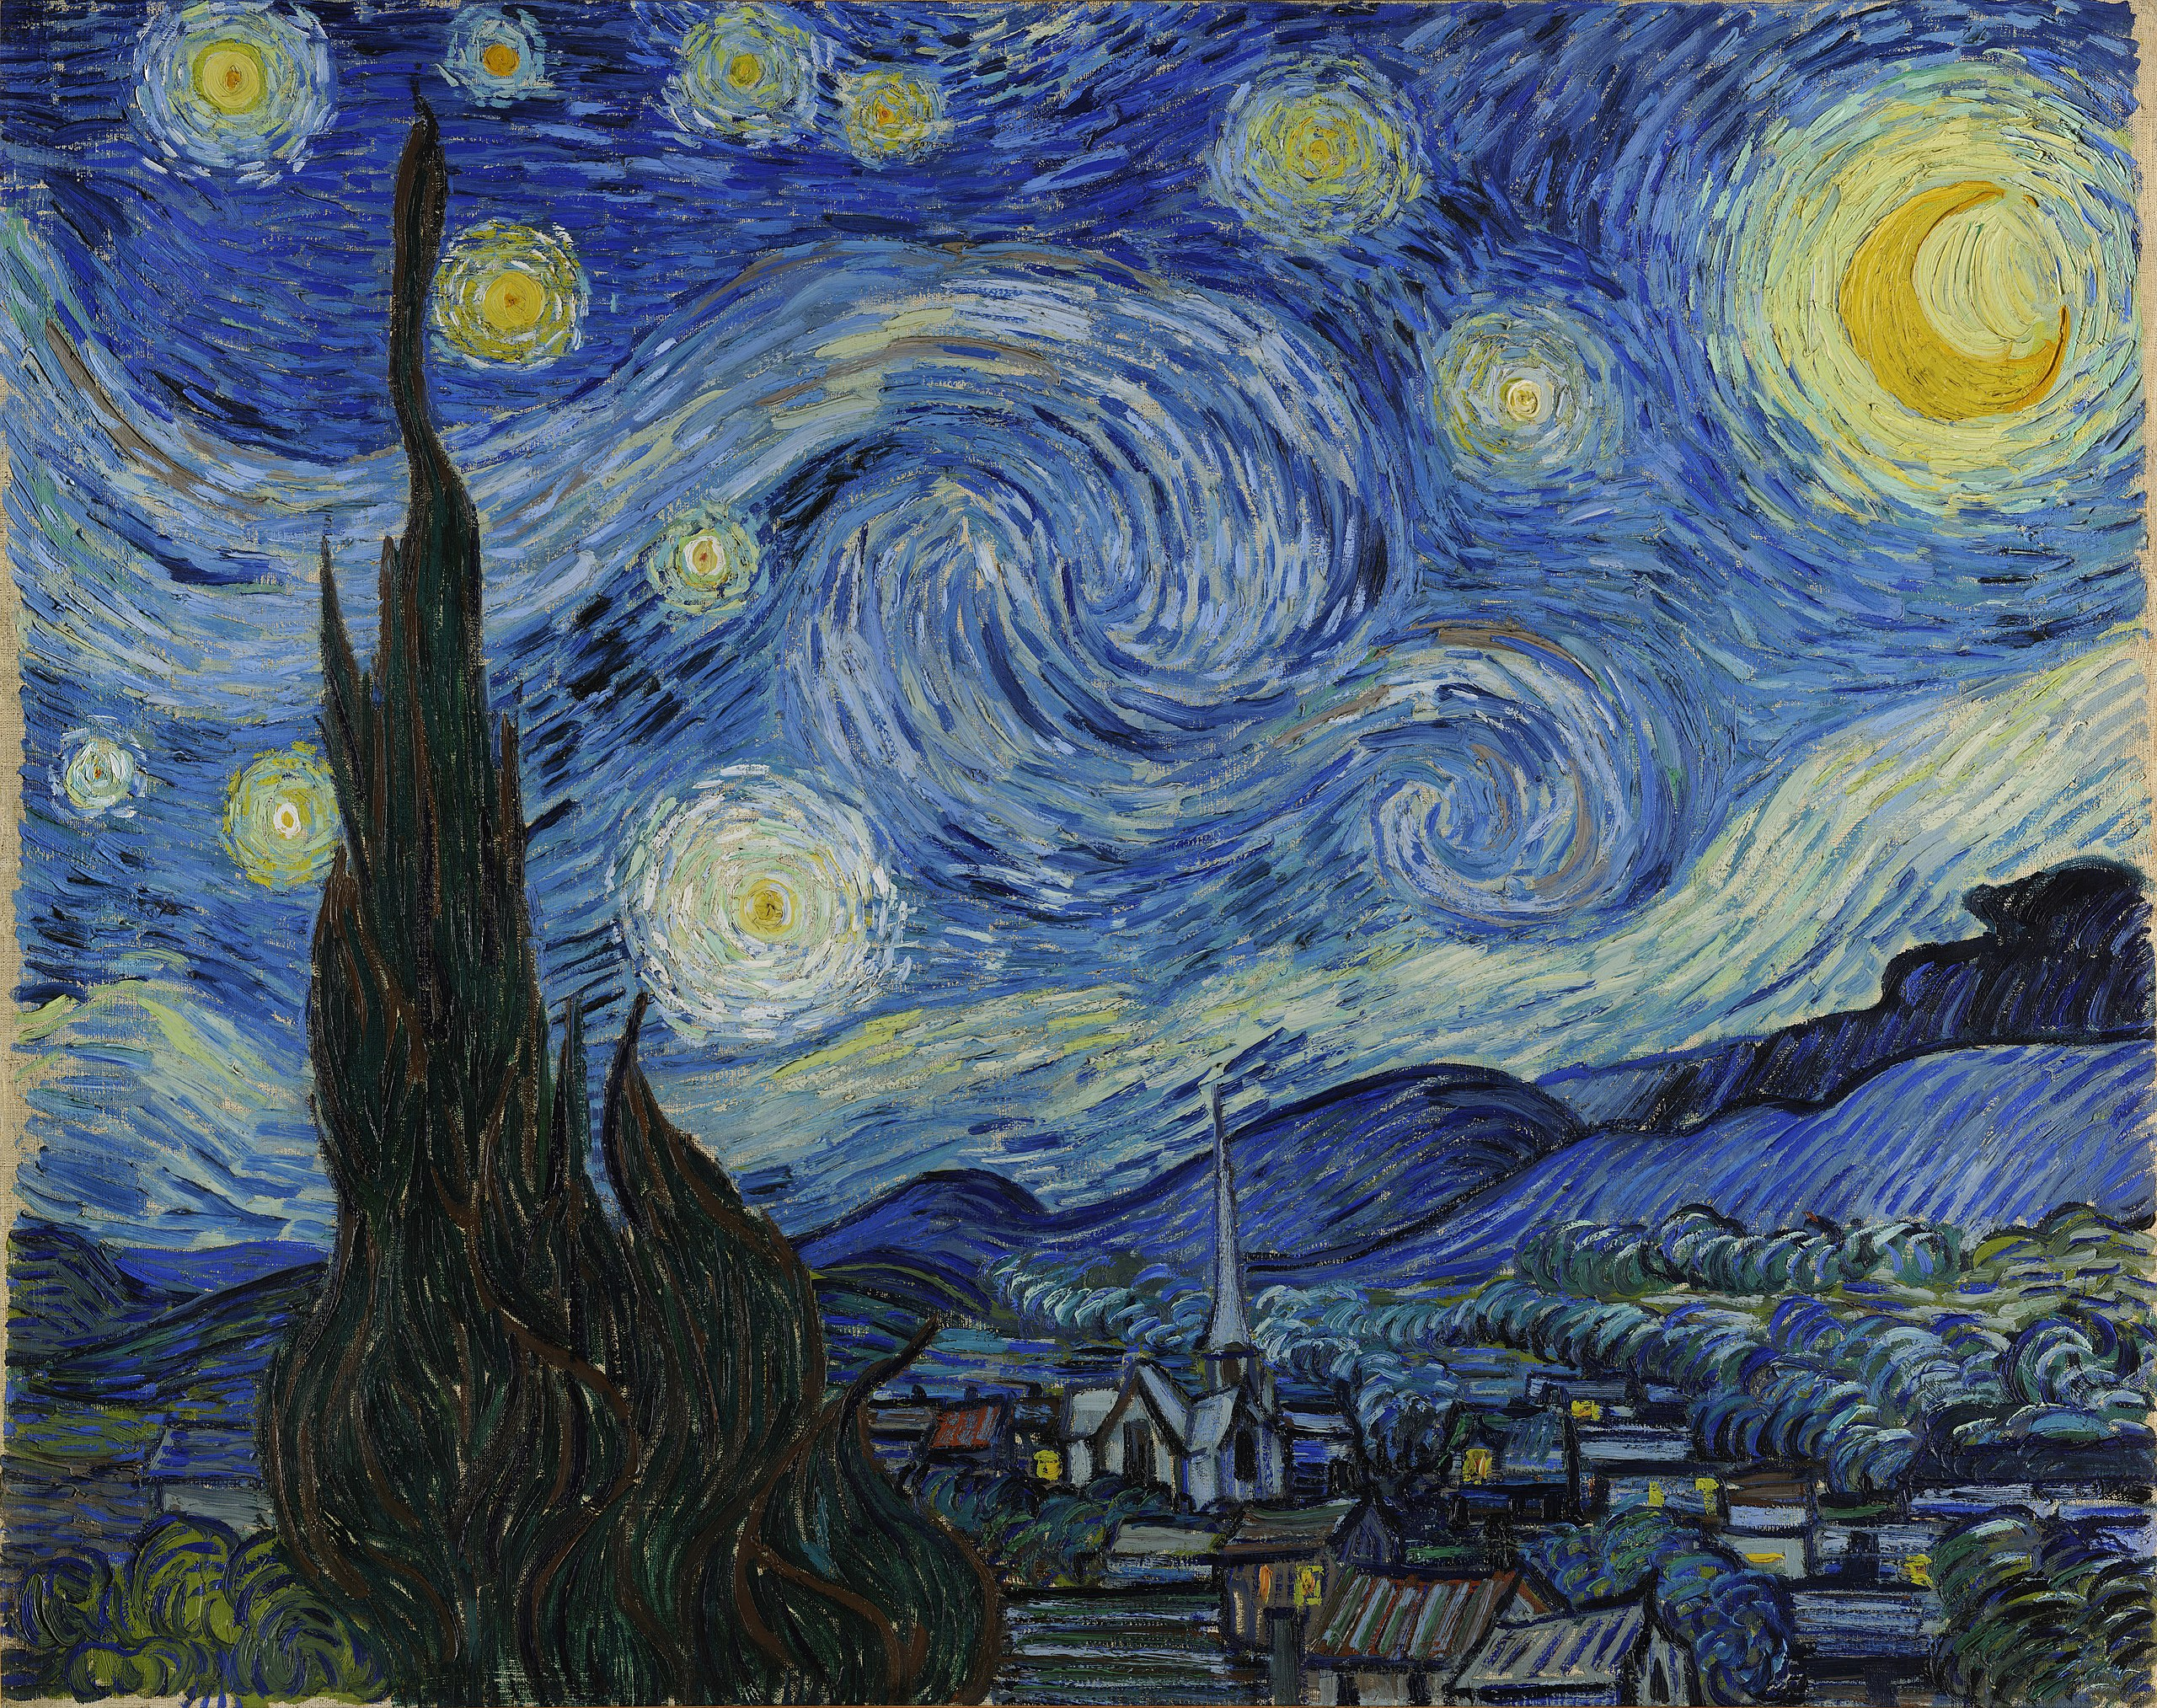
\includegraphics{figures/paintingexamples/starrynight}}
\caption{Like it or not, a continuous relation $[0,1] \rightarrow \blacksquare$: "The Starry Night", by Vincent van Gogh.}
\end{marginfigure}

\section{The category \textbf{TopRel}}

\begin{proposition}
Topological relations form a category $\mathbf{TopRel}$.
\begin{proof}
\newthought{Identities:} Identity relations, which are always topological.

\newthought{Composition:} The normal composition of relations. We verify that the composite $X^\tau \overset{R}{\rightarrow} Y^\sigma \overset{S}{\rightarrow} Z^\theta$ of continuous relations is again continuous as follows:
\[U \in \theta \implies S^\dag(U) \in \sigma \implies R^\dag \circ S^\dag(U) = (S \circ R)^\dag \in \tau\]

\newthought{Associativity of composition:} Inherited from \textbf{Rel}.
\end{proof}
\end{proposition}

\section{Biproducts}

We exhibit a free-forgetful adjunction between \textbf{Rel} and \textbf{TopRel}.

\begin{defn}[F: $\mathbf{Rel} \rightarrow \mathbf{TopRel}$] We define the action of the functor $F$:
\begin{description}
\item[On objects] $F(X) := X^\star$, ($X$ with the discrete topology)
\item[On morphisms] $F(X \overset{R}{\rightarrow} Y) := X^\star \overset{R}{\rightarrow} Y^\star$. Recall that any relation between sets is continuous with respect to the discrete topology.
\end{description}
Evidently identities and associativity of composition are preserved.
\end{defn}

\begin{defn}[U: $\mathbf{TopRel} \rightarrow \mathbf{Rel}$]
\begin{description} We define the action of the functor $U$:
\item[On objects] $U(X^\tau) := X$
\item[On morphisms] $U(X^\tau \overset{R}{\rightarrow} Y^\sigma) := X \overset{R}{\rightarrow} Y$
\end{description}
Evidently identities and associativity of composition are preserved.
\end{defn}

\begin{proposition}[$F \dashv U \dashv F$]
\begin{proof}

By triangular identities.

The composite $FU$ is precisely equal to the identity functor on $\mathbf{Rel}$. The unit natural transformation $1_\mathbf{Rel} \Rightarrow FU$ we take to be the identity morphisms.

\[\eta_{X} := \text{id}_{X}\]

The counit natural transformation $UF \Rightarrow 1_{\mathbf{TopRel}}$ we define:

\[\epsilon_{X^\tau} : X^\star \rightarrow X^\tau := \{(x,x) : x \in X\}\]

Now we verify the triangle identities

\[\]

\end{proof}
\end{proposition}

\begin{corollary}
$\mathbf{TopRel}$ has a zero object and biproducts.
\begin{proof}

\end{proof}
\end{corollary}

\section{Symmetric Monoidal Closed structure}

\marginnote{
\begin{rem}[Product Topology]
We denote the product topology of $X^\tau$ and $Y^\sigma$ as $(X \times Y)^{(\tau \times \sigma)}$. $\tau \times \sigma$ is the topology on $X \times Y$ generated by the basis $\{t \times s : t \in \mathfrak{b}_\tau, s \in \mathfrak{b}_\sigma\}$, where $\mathfrak{b}_\tau$ and $\mathfrak{b}_\sigma$ are bases for $\tau$ and $\sigma$ respectively.
\end{rem}
}

\begin{proposition}
$(\mathbf{TopRel},\{\star\}^{\bullet},X^\tau \otimes Y^\sigma := (X \times Y)^{(\tau \times \sigma)})$ is a symmetric monoidal closed category.
\begin{proof}

\newthought{Tensor Unit:} The one-point space $\bullet$. Explicitly, $\{\star\}$ with topology $\{\varnothing,\{\star\}\}$.

\marginnote{
    \begin{rem}[Product of relations]
    For relations between sets $R: X \rightarrow Y, S: A \rightarrow B$, the product relation $R \times S: X \times A \rightarrow Y \times B$ is defined to be \[ \{ ((x,a),(y,b)) : (x,y) \in R, (a,b) \in S \} \]
    \end{rem}
}

\newthought{Tensor Product:} For objects, $X^\tau \otimes Y^\sigma$ has base set $X \times Y$ equipped with the product topology $\tau \times \sigma$. For morphisms, $R \otimes S$ the product of relations. We show that the tensor of continuous relations is again a continuous relation. Take continuous relations $R: X^\tau \rightarrow Y^\sigma$, $S: A^\alpha \rightarrow B^\beta$, and let $U$ be open in the product topology $(\sigma \times \beta)$. We need to prove that $(R \times S)^\dag(U) \in (\tau \times \alpha)$. We may express $U$ as $\bigcup\limits_{i \in I} y_i \times b_i$, where the $y_i$ and $b_i$ are in the bases $\mathfrak{b}_\sigma$ and $\mathfrak{b}_\beta$ respectively. Since for any relations we have that $R(A \cup B) = R(A) \cup R(B)$ and $(R \times S)^\dag = R^\dag \times S^\dag$:

\begin{align*}
&(R \times S)^\dag(\bigcup\limits_{i \in I} y_i \times b_i)\\
 &= \bigcup\limits_{i \in I}(R \times S)^\dag(y_i \times b_i)\\
 &= \bigcup\limits_{i \in I}(R^\dag \times S^\dag)(y_i \times b_i)
 \end{align*}

Since each $y_i$ is open and $R$ is continuous, $R^\dag(y_i) \in \tau$. Symmetrically, $S^\dag(b_i) \in \alpha$. So each $(R^\dag \times S^\dag)(y_i \times b_i) \in (\tau \times \alpha)$. Topologies are closed under arbitrary union, so we are done.

\newthought{Unitors:} The left unitors $\lambda_{X^{\tau}}: \bullet \times X^\tau \rightarrow X^\tau$ maps $(\star,x) \mapsto x$, and we reverse the direction of the mapping to obtain the inverse $\lambda^{-1}_{X^{\tau}}$. The construction is symmetric for the right unitors $\rho_{X^{\tau}}$. 

\newthought{Associators:}

The associators $\alpha_{X^{\tau},Y^{\sigma},Z^{\rho}}$

\newthought{Braids:}


\newthought{Coherences:}



\end{proof}
\end{proposition}

\begin{fullwidth}

\section{\textbf{TopRel} diagrammatically}

\subsection{Relations that are always continuous}

\newthought{Here are five continuous relations for any $X^\tau$:}

\[\scalebox{0.75}{\tikzfig{bestiary/generators}}\]

\newthought{Copy and delete obey the following equalities:}

\[\scalebox{0.75}{\tikzfig{bestiary/basicrelations}}\]

\newthought{The copy map can also be used to distinguish the deterministic maps -- points and functions -- which we notate with an extra dot.}

\[\scalebox{0.75}{\tikzfig{structure/determinism}}\]

\newthought{Everything, delete, nothing-states and nothing-tests combine to give two numbers, one and zero.} There are extra expressions in grey squares above: they anticipate the tape-diagrams we will later use to graphically express another monoidal product of \textbf{TopRel}, the direct sum $\oplus$.

\[\scalebox{0.75}{\tikzfig{bestiary/scalarrelations}}\]

\newthought{Zero scalars turn entire diagrams into zero morphisms.} There is a zero-morphism for every input-output pair of objects in \textbf{TopRel}. 

\[\scalebox{0.75}{\tikzfig{bestiary/zerorelations}}\]

\section{Populating space with shapes using sticky spiders}

\begin{figure}\label{fig:spiderbicate}
\scalebox{0.7}{\tikzfig{bestiary/spiderbicat}}
\caption{The generators (in dashed boxes) and relations that make a spider. When the spider satisfies in addition the three inequalities b1-3, we call it a \textbf{relation-spider}.}
\end{figure}

\end{fullwidth}

\newpage

\subsection{When does an object have a spider (or something close to one)?}

\marginnote{
\begin{rem}[copy-compare spiders of $\mathbf{Rel}$]
For a set $X$, the \emph{copy} map $X \rightarrow X \times X$ is defined:
\[\{(x,(x,x)) : x \in X \}\]
the \emph{compare} map $X \times X \rightarrow X$ is defined:
\[\{((x,x),x) : x \in X \}\]
These two maps are the (co)multiplications of special frobenius algebras. The (co)units are \emph{delete}:
\[\{(x,\star) : x \in X\}\]
and \emph{everything}:
\[\{(\star,x) : x \in X\}\]
\end{rem}
}

\begin{example}[The copy-compare spiders of $\mathbf{Rel}$ are not always topological]\label{ex:compnotspider}
The compare map for the Sierpi\'{n}ski space is not topological, because the preimage of $\{0,1\}$ is $\{(0,0),(1,1)\}$, which is not open in the product space of $\mathcal{S}$ with itself.
\end{example}

\begin{proposition}\label{prop:copydiscrete}
The copy map is a spider iff the topology is discrete.
\begin{proof}
Discrete topologies inherit the usual copy-compare spiders from \textbf{Rel}, so we have to show that when the copy map is a spider, the underlying wire must have a discrete topology. Suppose that some wire has a spider, and construct the following open set using an arbitrary point $p$:
\[\scalebox{0.5}{\tikzfig{structure/copyspiderproof/openpoint}}\]
It will suffice to show that this open set is the singleton $\{p\}$ -- when all singletons are open, the topology is discrete. As a lemma, using frobenius rules and the property of zero morphisms, we can show that comparing distinct points $p \neq q$ yields the $\varnothing$ state.
\[\scalebox{0.5}{\tikzfig{structure/copyspiderproof/openpointproof}}\]
The following case analysis shows that our open set only contains the point $p$.
\[\scalebox{0.5}{\tikzfig{structure/copyspiderproof/openpointcases}}\]
\end{proof}
\end{proposition}

\marginnote{
    \begin{rem}[Split idempotents]
    An \textbf{idempotent} in a category is a map $e: A \rightarrow A$ such that \[A \overset{e}{\rightarrow} A \overset{e}{\rightarrow} A = A \overset{e}{\rightarrow} A\]
    A \textbf{split idempotent} is an idempotent $e: A \rightarrow A$ along with a \textbf{retract} $r: A \rightarrow B$ and a \textbf{section} $s: B \rightarrow A$ such that:
    \[A \overset{e}{\rightarrow} A = A \overset{r}{\rightarrow} B \overset{s}{\rightarrow} A\]
    \[B \overset{s}{\rightarrow} A \overset{r}{\rightarrow} B = B \overset{\mathop{id}}{\rightarrow} B\]
    \end{rem}
}

\begin{fullwidth}

\newthought{We can use split idempotents to transform copy-spiders from discrete topologies to almost-spiders on other spaces.} We can graphically express the behaviour of a split idempotent $e$ as follows, where the semicircles for the section and retract $r,s$ form a visual pun.

\[\scalebox{1}{\tikzfig{structure/idemspider/splitidem}}\]

\newthought{An idempotent on $Y^\sigma$ that splits through a discrete topology $X^\star$ does these things:}
\begin{description}
\item[The section:]{picks a subset of $s(x) \subseteq Y$ for each point $x \in X$. In order to be a split idempotent, $s(x)$ must be distinct for distinct points $x$.}
\item[The retract:]{(reading backwards) picks an open set $r(x) \in \sigma$ for each point $x \in X$. In order to be a split idempotent, $r(x)$ only overlaps $s(x)$ out of all other selected shapes: \[r(x) \cap s(x') = 1 \iff x = x'\]}
\end{description}
The combined effect is that the shapes $s(x)$ become copiable elements of the sticky spider, just as the points are the copiable elements of a regular spider.

\begin{defn}[Sticky spiders]
A \textbf{sticky spider} (or just an $e$-spider, if we know that $e$ is a split idempotent), is a spider \emph{except} every identity wire on any side of an equation in Figure \ref{fig:spiderbicate} is replaced by the idempotent $e$.
\[\scalebox{1}{\tikzfig{structure/idemspider/espiderproperties}}\]
\[\scalebox{1}{\tikzfig{structure/idemspider/espiderproperties2}}\]

The desired graphical behaviour of a sticky spider is that one can still coalesce all connected spider-bodies together, but the 1-1 spider "sticks around" rather than disappearing as the identity. This is achieved by the following rules that cohere the idempotent $e$ with the (co)unit and (co)multiplications.

\[placeholder\]
\end{defn}

\begin{construction}[Sticky spiders from split idempotents]
Given an idempotent $e: Y^\sigma \rightarrow Y^\sigma$ that splits through a discrete topology $X^\star$, we construct a new (co)multiplication as follows:
\[\scalebox{1}{\tikzfig{structure/idemspider/idemspiderv2}}\]
\end{construction}

\begin{proposition}[Every idempotent that splits through a discrete topology gives a sticky spider]\label{prop:splitmeanssticky}
\[\scalebox{1}{\tikzfig{structure/idemspider/espiderstatement}}\]
\begin{proof}
We can check that our construction satisfies the frobenius rules as follows. We only present one equality; the rest follow the same idea.
\[\scalebox{1}{\tikzfig{structure/idemspider/espiderproofv2}}\]
To verify the sticky spider rules, we first observe that since \[X^\star \overset{s}{\rightarrow} Y^\sigma \overset{r}{\rightarrow} X^\star = X^\star \overset{\mathop{id}}{\rightarrow} X^\star\]
$r$ must have all of $X^\star$ in its image, and $s$ must have all of $X^\star$ in its preimage, so we have the following:
\[\scalebox{1}{\tikzfig{structure/idemspider/splitonto}}\]
Now we show that e-unitality holds:
\[\scalebox{1}{\tikzfig{structure/idemspider/espiderproof2}}\]
The proofs of e-counitality, and e-speciality follow similarly.
\end{proof}
\end{proposition}

\newthought{We can prove a partial converse of Proposition \ref{prop:splitmeanssticky}:} we can identify two diagrammatic equations that tell us precisely when a sticky spider has an idempotent that splits though some discrete topology.

\begin{theorem}\label{thm:stickygraphical}
A sticky spider has an idempotent that splits through a discrete topology if and only if in addition to the sticky spider equalities, the following relations are also satisfied.
\[\scalebox{1}{\tikzfig{idemproof/unit-everything}} \quad\quad\quad\quad \scalebox{1}{\tikzfig{idemproof/comult-copy}}\]
\end{theorem}

\[\scalebox{0.75}{\tikzfig{idemproof/claimmap2}}\]

\begin{proposition}[comult/copy implies counit/delete]\label{prop:counitdelete}
\[\scalebox{1}{\tikzfig{idemproof/ecopy2delclaim}}\]
\begin{proof}
\[\scalebox{1}{\tikzfig{idemproof/ecopy2del}}\]
\end{proof}
\end{proposition}

\newpage
\begin{lemma}[All-or-Nothing]\label{lem:allornothing}
Consider the set $e(\{x\})$ obtained by applying the idempotent $e$ to a singleton $\{x\}$, and take an arbitrary element $y \in e(x)$ of this set. Then $e(\{y\}) = \varnothing$ or $e(\{x\}) = e(\{y\})$. Diagrammatically: \[\scalebox{0.75}{\tikzfig{idemproof/allornothingclaim}}\]
\begin{proof}
\[\scalebox{0.75}{\tikzfig{idemproof/allornothing2a}}\]
\[\scalebox{0.75}{\tikzfig{idemproof/allornothing2b}}\]
\end{proof}
\end{lemma}

\begin{proposition}[$e$ of any point is $e$-copiable]\label{prop:epointcopy}
\[\scalebox{0.75}{\tikzfig{idemproof/pointidemcopiable}}\]
\begin{proof}
\[\scalebox{0.75}{\tikzfig{idemproof/pointidemcopiableproof}}\]
\end{proof}
\end{proposition}

\begin{proposition}[The unit is the union of all $e$-copiables]\label{prop:copiablebasis}
\[\scalebox{1}{\tikzfig{idemproof/copiablebasisclaim}}\]
\begin{proof}
\[\scalebox{1}{\tikzfig{idemproof/copiablebasis}}\]
\end{proof}
\end{proposition}

\begin{proposition}[$e$-copiable decomposition of $e$]\label{prop:decompidem}
\[\scalebox{1}{\tikzfig{idemproof/decompidemclaim}}\]
\begin{proof}
\[\scalebox{1}{\tikzfig{idemproof/decompidem}}\]
\end{proof}
\end{proposition}

\begin{proposition}[$e$-copiable decomposition of counit]\label{prop:decompcounit}
\[\scalebox{1}{\tikzfig{idemproof/decompcounitclaim}}\]
\begin{proof}
\[\scalebox{1}{\tikzfig{idemproof/decompcounit}}\]
\end{proof}
\end{proposition}

\newthought{The $e$-copiable states really do behave like an orthonormal basis, as the following Lemmas show.}

\begin{lemma}[$e$-copiables are orthogonal under multiplication]\label{lem:match}
\[\scalebox{1}{\tikzfig{idemproof/matchclaim}}\]
\begin{proof}
\[\scalebox{0.9}{\tikzfig{idemproof/match}}\]
\end{proof}
\end{lemma}

\begin{convention}[Shorthand for the open set associated with an $e$-copiable]
We introduce the following diagrammatic shorthand.
\[\scalebox{1}{\tikzfig{idemproof/openshorthand}}\]
Including the coloured dot is justified, because these open sets are co-copiable with respect to the multiplication of the sticky spider.
\[\scalebox{1}{\tikzfig{idemproof/shorthandjustification}}\]
\end{convention}

\begin{lemma}[Co-match]\label{lem:comatch}
\[\scalebox{1}{\tikzfig{idemproof/comatchclaim}}\]
\begin{proof}
\[\scalebox{0.9}{\tikzfig{idemproof/comatch}}\]
The claim then follows by applying Lemma \ref{lem:match} to the final diagram.
\end{proof}
\end{lemma}

\begin{lemma}[e-copiables are e-fixpoints]\label{lem:ecopyfixpoint}
\[\scalebox{1}{\tikzfig{idemproof/dotcopyableclaim}}\]
\begin{proof}
\[\scalebox{1}{\tikzfig{idemproof/dotcopyable}}\]
Observe that the final equation of the proof also holds when the initial e-copiable is the empty set.
\end{proof}
\end{lemma}

\begin{lemma}[$e$-copiables are normal]\label{lem:ecopynormal}
\[\scalebox{1}{\tikzfig{idemproof/copynormalclaim}}\]
\begin{proof}
\[\scalebox{1}{\tikzfig{idemproof/copynormal}}\]
\end{proof}
\end{lemma}
{}
\begin{proposition}[$e$-copiable decomposition of multiplication]\label{prop:decompmult}
\[\scalebox{1}{\tikzfig{idemproof/decompmultclaim}}\]
\begin{proof}
\[\scalebox{1}{\tikzfig{idemproof/decompmult}}\]
\end{proof}
\end{proposition}

\begin{proposition}[$e$-copiable decomposition of comultiplication]\label{prop:decompcomult}
\[\scalebox{1}{\tikzfig{idemproof/decompcomultclaim}}\]
\begin{proof}
\[\scalebox{1}{\tikzfig{idemproof/decompcomult}}\]
\end{proof}
\end{proposition}

\newthought{Now we can prove Theorem \ref{thm:stickygraphical}.}
\begin{proof}
The key observation is that the $e$-copiable decomposition of the idempotent given by Proposition \ref{prop:decompidem} is equivalent to a split idempotent though the set of $e$-copiables equipped with discrete topology.
\[placeholder\]

\end{proof}

\end{fullwidth}

\section{Shapes: cores, halos, and parthood}

\begin{defn}[Shape]
Shapes are a core and a halo.
\end{defn}

\begin{defn}[Core]
Cores are open sets.
\end{defn}

\begin{defn}[Halo]
\end{defn}

\begin{lemma}[Interactions between cores and halos in a sticky spider]\label{lem:corehalo} The following hold for all sticky spiders:\\
\begin{enumerate}
\item{Cores never overlap}
\item{Each core overlaps with exactly one halo}
\end{enumerate}
\end{lemma}

\begin{example}[Discrete Quantum Venn Diagram Paradox]

\end{example}

\begin{defn}[Parts]
When a core of a shape is equal to its halo, we call the shape a \textbf{part}. By Lemma \ref{lem:corehalo}, parts are open sets that do not overlap with any other core or halo.
\end{defn}

\begin{defn}[Mereology]
 When all the cores of a sticky spider are equal to their parts, we call the spider a \textbf{mereology}: a theory of parthood relations. A mereology on a topology $X^\tau$ is a collection of mutually disjoint open sets of $X^\tau$. Conversely, every such collection of disjoint open sets yields a mereology; the idempotent splits through the set of disjoint opens equipped with the discrete topology.
\end{defn}

\begin{proposition}[Mereologies, graphically]
A sticky spider is a mereology -- every core of the sticky spider is equal to its corresponding halo -- if and only if the following equation holds:\marginnote{\textbf{TopRel} does not have a dagger functor, so this equation is an approximation of the concept of a dagger-special-frobenius-algebra.}
\[\scalebox{1}{\tikzfig{idemproof/mereology}}\]
\end{proposition}

\begin{example}[Parts as places on a map]

\end{example}

\section{Displacing shapes with symmetries}

\begin{defn}[Topological Group]

\end{defn}

\begin{defn}[Sticky spiders equivalent up to symmetric displacement]

\end{defn}

\section{Moving shapes with homotopies}



\section{Stage-spaces from sticky spiders}

\begin{defn}[The stage-space of a sticky spider]

\end{defn}

\begin{defn}[The "interaction" relation]

\end{defn}

\begin{defn}[Movement equivalence classes]

\end{defn}

\section{Topological models for a selection of concepts}

\begin{construction}[Putting-in and getting-out things from containers]

\end{construction}

\begin{construction}[Filling holes, fullness, and fitting]

\end{construction}

\begin{construction}[Sending by throwing and conduits]

\end{construction}

\begin{construction}[Conduit Metaphor]

\end{construction}

\begin{construction}[Locks and labyrinths]

\end{construction}

\begin{fullwidth}
\section{Modelling Lassos and the Universal Object of Monoidal Computer}

Recall that Lassos -- a graphical gadget that can encode arbitrary morphisms into a single wire -- can be interpreted in a monoidal computer. Recall that monoidal computers require a universal object $\Xi$. Here we show how in \textbf{TopRel}, by taking $\Xi := \squarehvfill$ the open unit square, we have a monoidal computer in \textbf{Rel} restricted to countable sets and the relations between them. We will make use of sticky spiders. We have to show that; $\squarehvfill$ has a sticky-spider corresponding to every countable set; how there is a suitable notion of sticky-spider morphism to establish a correspondence with relations; what the continuous relations are on $\squarehvfill$ that mimick various compositions of relations.

\begin{proposition}[$(0,1) \times (0,1)$ splits through any countable set $X$]
For any countable set $X$, the open unit square $\squarehvfill$ has a sticky spider that splits through $X^\star$.
\begin{proof}
The proof is by construction. We'll assume the sticky-spiders to be mereologies, so that cores and halos agree. Then we only have to highlight the copiable open sets. Take some circle and place axis-aligned open squares evenly along them, one for each element of $X$. The centres of the open squares lie on the circumference of the circle, and we may shrink each square as needed to fit all of them.
\[\scalebox{1}{\tikzfig{spatialencoding/circencodingconstruct}}\]
\end{proof}
\end{proposition}

\begin{defn}[Morphism of sticky spiders]
A morphism between sticky spiders is any morphism that satisfies the following equation.
\[\scalebox{1}{\tikzfig{spatialencoding/stickymorphismdefn}}\]
\end{defn}

\begin{proposition}[Morphisms of sticky spiders encode relations]
For arbitrary split idempotents through $A^\star$ and $B^\star$, the morphisms between the two resulting sticky spiders are in bijection with relations $R: A \rightarrow B$.
\[\scalebox{1}{\tikzfig{spatialencoding/arbsetclaim}}\]
\begin{proof}
\[\scalebox{1}{\tikzfig{spatialencoding/arbset}}\]
\end{proof}
\end{proposition}

\begin{construction}[Representing sets in their various guises within $\squarehvfill$]
We can represent the direct sum of two $\squarehvfill$-representations of sets as follows.
\[\scalebox{1}{\tikzfig{spatialencoding/directsumconstruct}}\]
The important bit of technology is the homeomorphism that losslessly squishes the whole unit square into one half of the unit square. The decompressions are partial continuous functions, with domain restricted to the appropriate half of the unit square.
\[\scalebox{1}{\tikzfig{spatialencoding/leftrightcompressions}}\]
We express the ability of these relations to encode and decode the unit square in just either half by the following graphical equations.
\[\scalebox{1}{\tikzfig{spatialencoding/leftrightcompressions2}}\]
Now, to put the two halves together and to take them apart, we introduce the following two relations. In tandem with the squishing and stretching we have defined, these will behave just as the projections and injections for the direct-sum biproduct in \textbf{Rel}.
\[\scalebox{1}{\tikzfig{spatialencoding/leftrightcompressions3}}\]
The following equation tells us that we can take any two representations in $\squarehvfill$, put them into a single copy of $\squarehvfill$, and take them out again. Banach and Tarski would approve.
\[\scalebox{1}{\tikzfig{spatialencoding/leftrightcompressions4}}\]
We encode the tensor product $A \otimes B$ of representations by placing copies of $B$ in each of the open boxes of $A$.
%\[\scalebox{0.75}{\tikzfig{spatialencoding/directsummap}}\]
%\[\scalebox{0.75}{\tikzfig{spatialencoding/directsummap2}}\]
\[\scalebox{1}{\tikzfig{spatialencoding/tensorconstruct}}\]
The important bit of technology here is a family of homeomorphisms of $\squarehvfill$ parameterised by axis-aligned open boxes. We depict the parameters outside the body of the homeomorphism for clarity. The squish is on the left, the stretch on the right.
\[\scalebox{1}{\tikzfig{spatialencoding/boxcompression}}\]
Now, for every representation of a set in $\squarehvfill$ by a sticky-spider, where each element corresponds to an axis-aligned open box, we can associate each element with a squish-stretch homeomorphism via the parameters of the open box, which we notate with a dot above the name of the element.
\[\scalebox{1}{\tikzfig{spatialencoding/obtainboxposition}}\]
Now we can define the "tensor $X$ on the left" relation $\_ \rightarrow X \otimes \_$ and its corresponding cotensor.
\[\scalebox{1}{\tikzfig{spatialencoding/tensordetensor}}\]
The tensor and cotensor behave as we expect from proof nets for monoidal categories.
\[\scalebox{1}{\tikzfig{spatialencoding/tensordetensor2}}\]
And by construction, the (co)tensors and (co)pluses interact as we expect, and they come with all the natural isomorphisms between representations we expect. For example, below we exhibit an explicit associator natural isomorphism between representations.
\[\scalebox{1}{\tikzfig{spatialencoding/tensordetensor3}}\]
\end{construction}

\begin{construction}[Representing relations between sets and their composition within $\squarehvfill$]
With all the above, we can establish a special kind of process-state duality; relations as processes are isomorphic to states of $\squarehvfill$, up to the representation scheme we have chosen.
\[\scalebox{1}{\tikzfig{spatialencoding/relcomp1}}\]
Moreover, we have continuous relations that perform sequental composition of relations.
\[\scalebox{1}{\tikzfig{spatialencoding/relcomp2}}\]
And we also know how to take the parallel composition of relations by tensors.
\[\scalebox{1}{\tikzfig{spatialencoding/relcomp3}}\]
\end{construction}

\end{fullwidth}

\end{document}